\section{Results and discussion}
\FloatBarrier
\subsection{Charge definitions produce element-dependent differences}
Charge definitions differ in both scale and direction across elements (Figure~\ref{fig:landscape}). The structure-balanced DDEC6--Bader mean is $-0.29096$~\charge\ for carbon and $+0.58916$~\charge\ for oxygen; the corresponding DDEC6--CM5 means are $+0.03938$ and $-0.23530$~\charge. Thus, the sign of an elementwise difference can reverse with the charge pair. These means describe the same aligned atomic sites, but an environment contrast could still reflect different sampling of an element-specific charge relation. The conditional models test what remains after that relation is supplied explicitly.

All three pairs use the same availability-defined cohort. Graph construction completed for all structures, while 24,297 atoms received diagnostic ambiguity flags. Keeping these sites in the atlas preserves the environments where an operational neighborhood assignment deserves closer inspection; it does not equate a flag with an incorrect bond.

\begin{figure}[!htbp]
\centering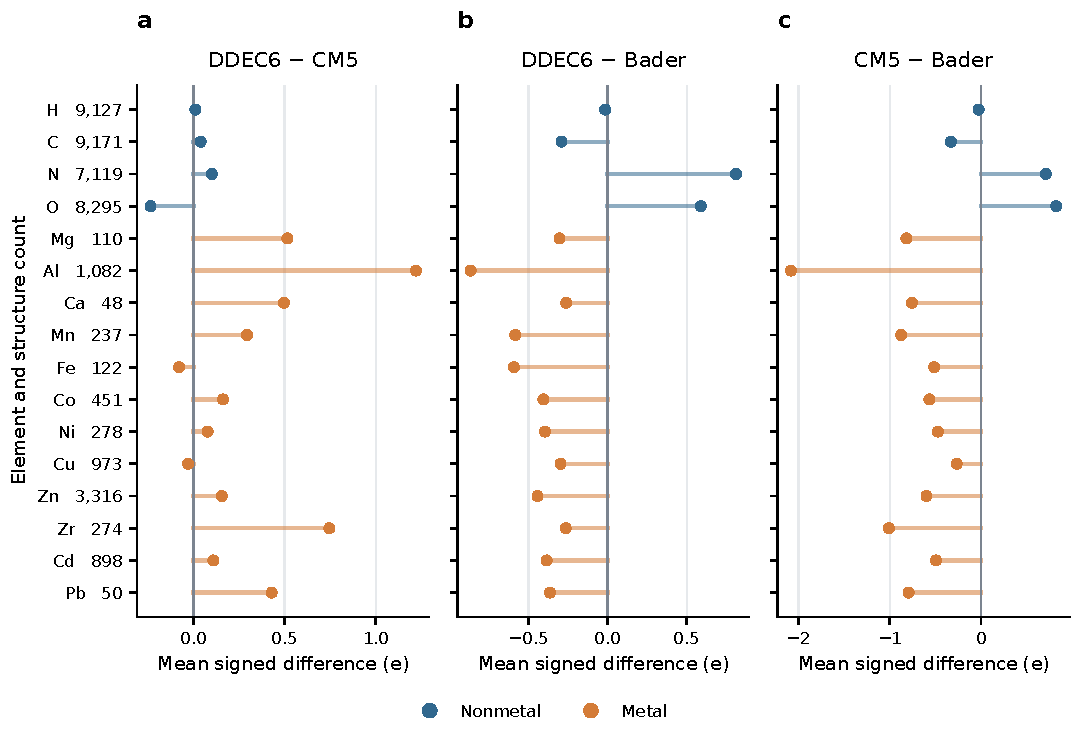
\includegraphics[width=\textwidth]{figures/Figure_01_charge_landscape.pdf}
\caption{\textbf{Element-dependent charge-definition disagreement.} Structure-balanced mean signed differences for 16 displayed elements in the 9,171-structure common cohort. Points are descriptive means; no uncertainty intervals are plotted. Each structure contributes equally within the stated element population. Orange marks metal elements and blue marks nonmetals under the operational classification. Counts beside the elements are numbers of represented structures; the same structure can contribute to multiple elements. Points describe charge definitions and are not errors relative to a reference charge. Complete distributions are retained with the numerical evidence.}
\label{fig:landscape}
\end{figure}

\FloatBarrier
\subsection{Local chemistry contributes beyond the tested charge-only mapping}
Adding local structural information reduces held-out error after a flexible relation between charge definitions has already been fitted (Figure~\ref{fig:conditional}). Under identifier/composition blocking, the charge-only to two-hop MAE decreases are 0.02434 to 0.01018~\charge\ for DDEC6--CM5, 0.08454 to 0.03885~\charge\ for DDEC6--Bader, and 0.06750 to 0.03914~\charge\ for CM5--Bader. Table~\ref{tab:main} reports the matched gains and paired intervals. The gains correspond to approximately 58\%, 54\%, and 42\% of charge-only MAE, respectively. Every all-atom gain is positive in all five folds under both validation schemes (Figure S3).

\begin{table}[!htbp]
\centering\small
\caption{Identifier/composition-blocked structure-balanced MAE and paired two-hop gain over charge only, in e. All 9,171 structures and 1,420,532 atoms are evaluated. Intervals are pointwise 95\% component-bootstrap intervals conditional on fitted models.}
\label{tab:main}
\setlength{\tabcolsep}{3pt}
\begin{tabular}{lrrrrl}
\toprule
Charge pair & Charge only & First shell & Two-hop & Gain & 95\% interval \\
\midrule
DDEC6--CM5 & 0.02434 & 0.01309 & 0.01018 & 0.01416 & [0.01400, 0.01432] \\
DDEC6--Bader & 0.08454 & 0.04197 & 0.03885 & 0.04569 & [0.04495, 0.04640] \\
CM5--Bader & 0.06750 & 0.03981 & 0.03914 & 0.02837 & [0.02782, 0.02893] \\
\bottomrule
\end{tabular}
\end{table}


Most of the reduction comes from the first shell, consistent with immediate chemical context carrying information that the source charge alone does not encode in these regressors. Two-hop paths then reduce blocked MAE by a further 0.00291, 0.00311, and 0.00068~\charge\ for the three ordered pairs, respectively. The smaller path increments indicate information beyond immediate neighbors. This is a comparison of fixed regressors: the gain quantifies the information recovered by these representations and controls, rather than exhausting every possible scalar mapping.

Related-record blocking leaves the principal result intact. The 1,414 records in nonsingleton components retain gains of 0.01306~\charge\ for DDEC6--CM5, 0.04664~\charge\ for DDEC6--Bader, and 0.02687~\charge\ for CM5--Bader, with intervals above zero. The improvement is therefore also present in the subset directly affected by grouping. However, exact formula and MOFkey blocking are conservative operational checks, not proof of transfer to wholly new linkers, metals, or topologies.

\begin{figure}[!htbp]
\centering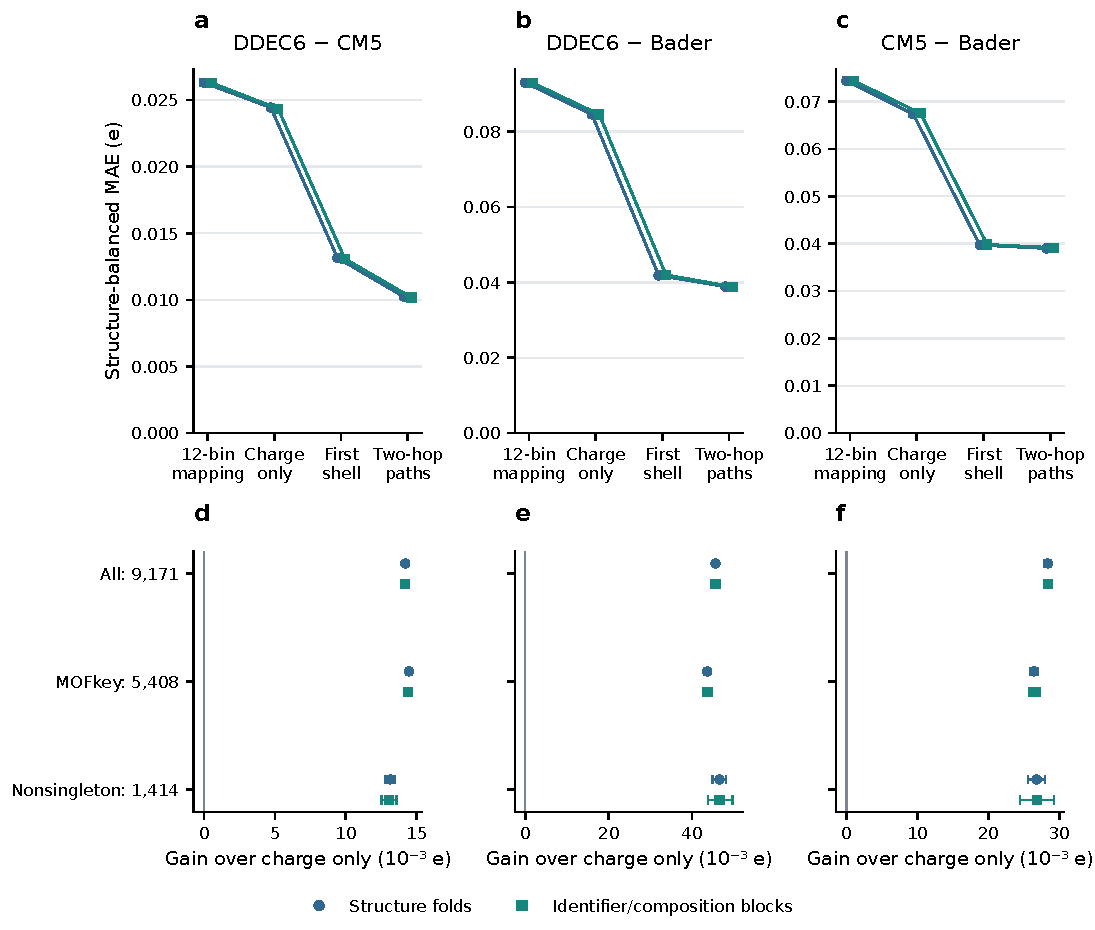
\includegraphics[width=\textwidth]{figures/Figure_02_conditional_evidence.pdf}
\caption{\textbf{Structural information survives charge conditioning and the specified blocking challenge.} (a--c) Structure-balanced held-out MAE for the training-fitted piecewise mapping, flexible charge-only tree, and nested first-shell and two-hop models, over all 9,171 structures and 1,420,532 atoms. All tree competitors share fitting atoms and weights. (d--f) Paired MAE gain of the two-hop model over the flexible charge-only model for all records, MOFkey-present records, and records in nonsingleton blocking components. The panels retain separate charge-pair scales. Error bars are pointwise 95\% bootstrap intervals, resampling structures or identifier/composition components as appropriate. Intervals condition on the fitted models.}
\label{fig:conditional}
\end{figure}

\FloatBarrier
\subsection{Directional shifts and larger departures are different chemical findings}
The environment atlas asks a complementary question: where do charge differences depart from the flexible charge-only relation? Figure~\ref{fig:contrasts} separates paired contrasts in signed residuals from paired contrasts in absolute residuals. Positive and negative signs refer to the fixed ordering $q^A-q^B$ and to the left environment minus the right environment. They are not oxidation-state changes.

O-attached carbon provides a clear distinction. Relative to strictly C/H-only carbon, the blocked DDEC6--Bader signed departure contrast is $-0.07210$~\charge\ (95\% interval $[-0.07491,-0.06946]$; 7,601 paired structures). The corresponding absolute-departure contrast is $-0.00112$~\charge\ with an interval spanning zero, $[-0.00342,0.00126]$. The directional shift therefore does not establish larger absolute disagreement in this contrast.

The converse occurs for N-attached, O-absent carbon in CM5--Bader. Across 6,689 paired structures, its signed contrast against C/H-only carbon is close to zero, $+0.00068$~\charge\ ($[-0.00378,0.00540]$), while its absolute-departure contrast is $+0.10216$~\charge\ ($[0.09904,0.10558]$). Cancellation in a signed summary can therefore coexist with a substantial difference in departure magnitude. The residual-spread contrasts also differ: O-attached carbon has a lower within-environment spread by 0.03488~\charge, whereas N-attached carbon has a higher spread by 0.03716~\charge\ in the respective comparisons. These are differences in averages of within-structure standard deviations, not pooled spreads or uncertainty in a physical charge. Figure S4 places these examples within the broader supported atlas.''

The size of a chemical contrast also depends on the scalar relation removed before constructing the atlas. For example, the original-fold DDEC6--CM5 N--H versus C--H signed contrast changes from approximately $-0.06788$~\charge\ after the earlier piecewise-only correction to $-0.02187$~\charge\ after the flexible charge-only correction. The persistence of a chemical contrast must therefore be evaluated against its stated control, not inferred from an unadjusted comparison. The atlas retains these distinctions, support counts, and ambiguity coverage; the full set includes weak and null contrasts.

\begin{figure}[!htbp]
\centering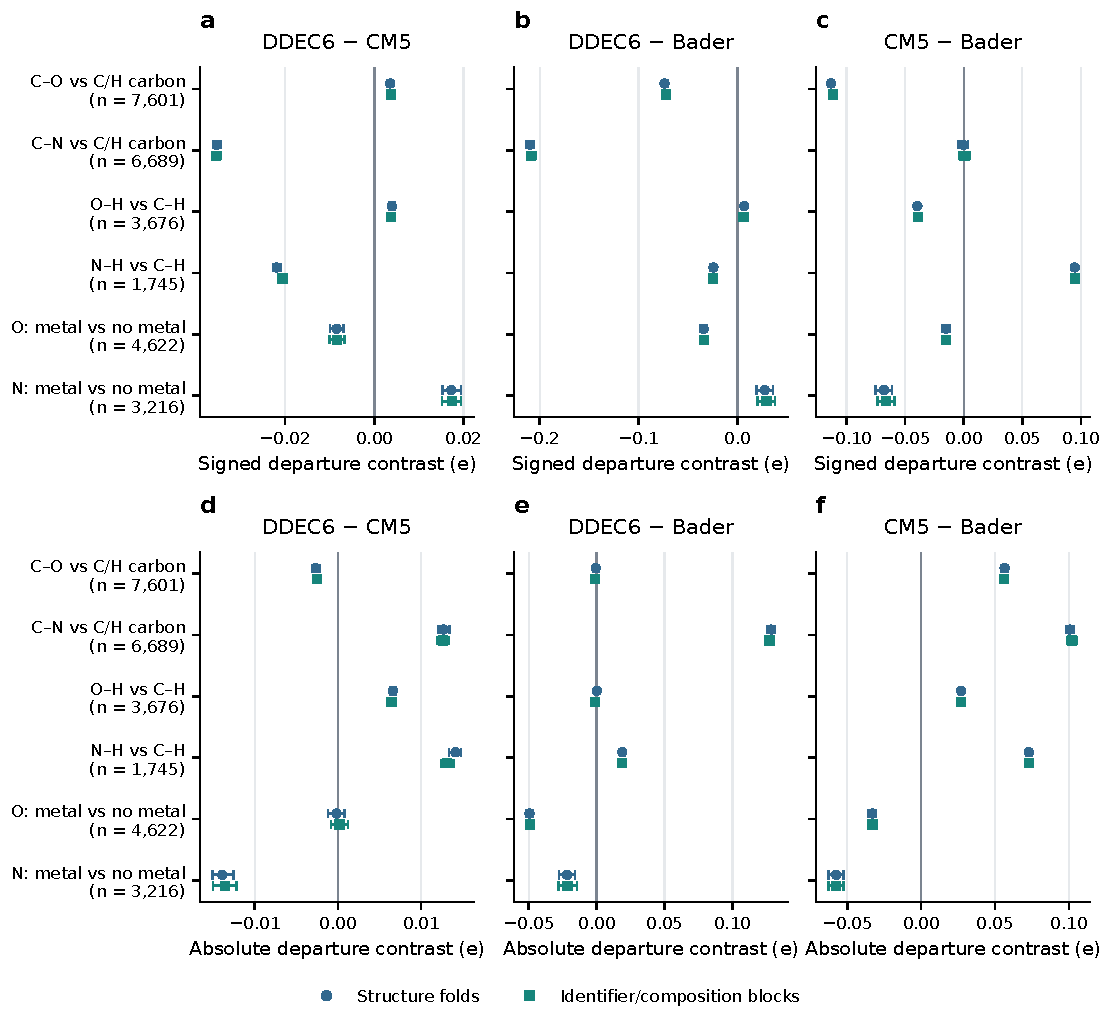
\includegraphics[width=\textwidth]{figures/Figure_03_chemical_contrasts.pdf}
\caption{\textbf{Chemical shifts do not imply larger absolute departures.} Paired within-structure contrasts after subtraction of the flexible charge-only held-out prediction. (a--c) Signed residual contrasts. (d--f) Absolute residual contrasts. Each row compares two environments of the same element within structures containing both classes; $n$ is the number of paired structures. C--N denotes N-attached, O-absent carbon; C/H carbon has only C/H neighbors. H classes require monocoordinate H. Metal adjacency follows the accepted graph. Points show the original and identifier/composition-blocked splits; error bars are pointwise 95\% paired bootstrap intervals, with no multiplicity adjustment. The three pair targets are algebraically related. These descriptive contrasts quantify empirical mapping departures rather than causal effects or physical charge error.}
\label{fig:contrasts}
\end{figure}

\FloatBarrier
\subsection{The all-atom result does not imply a general central-metal benefit}
Metal-centered predictions give a more qualified result (Figure~\ref{fig:metal}). Across 46,994 metal atoms in 9,165 structures, adding local structural features to the global conditional model improves blocked DDEC6--CM5 MAE from approximately 0.02694 to 0.02202~\charge. The gain is 0.00493~\charge\ ($[0.00451,0.00533]$). CM5--Bader shows a much smaller gain, 0.00091~\charge\ ($[0.00049,0.00137]$).

For DDEC6--Bader, the same comparison worsens metal MAE from approximately 0.02044 to 0.02851~\charge. The negative gain, $-0.00807$~\charge\ ($[-0.00857,-0.00749]$), occurs in all five blocked folds. This failure is not removed by the strong all-atom result. A global fitting population can capture the dominant nonmetal pattern while giving a different result at metal centers. Metals constitute only about 3.3\% of the atoms, so aggregate success can coexist with deterioration at their centers. Structure balancing prevents large structures from dominating the metric, but does not make a global training population equivalent to a metal-specific one. The earlier metal-only model is reported separately as a follow-up to a global failure; it does not replace this conditional result.

\begin{figure}[!htbp]
\centering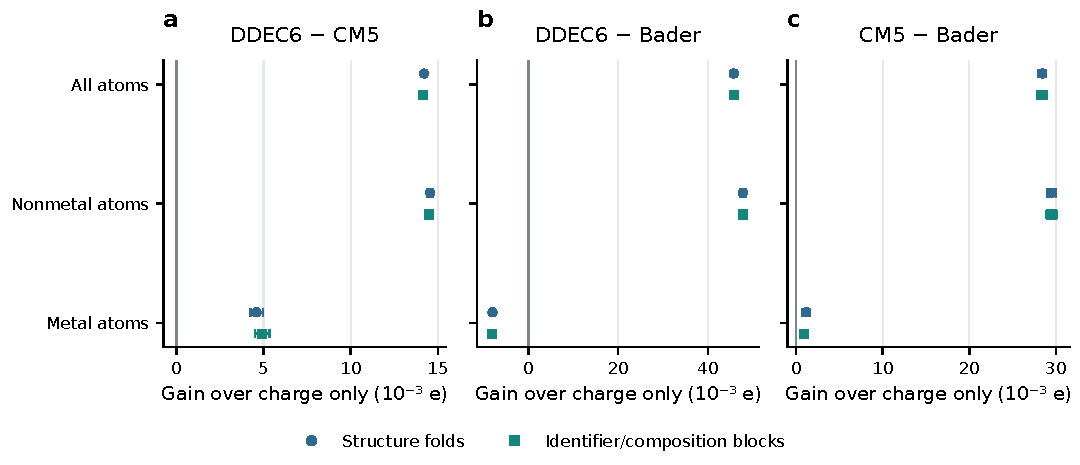
\includegraphics[width=\textwidth]{figures/Figure_04_population_limits.pdf}
\caption{\textbf{Population-specific limits of the conditional result.} MAE gain of the two-hop conditional model over the flexible charge-only model for all atoms, nonmetal atoms, and central metal atoms. Positive values favor the structural model; negative values indicate worse prediction. Original and identifier/composition-blocked fits are shown separately with pointwise 95\% paired bootstrap intervals. The global DDEC6--Bader metal failure is retained. The metal population is 46,994 atoms in 9,165 structures; population means weight represented structures equally. Panels use separate horizontal scales; the small CM5--Bader metal gain should not be equated with the larger all-atom gains.}
\label{fig:metal}
\end{figure}

\FloatBarrier
\subsection{Connectivity uncertainty bounds the chemical interpretation}
The graph determines which local environment is assigned to an atom. Its influence must therefore be distinguished from charge-definition disagreement itself. On the fixed 96-structure subset, lowering the nonmetal radius scale from 1.25 to 1.20 changes no first shells. Raising it to 1.30 adds 12 image-aware, unoriented contacts and changes 18 first-shell and 38 two-hop feature records. The six tested headline environment memberships and their common-pair contrasts remain unchanged on this subset (Figure~\ref{fig:graph}; Figure S5).

The wider cutoff nevertheless exposes a chemically meaningful ambiguity. Six H sites lie close to the midpoint of nearly linear O--H--O arrangements, with added H--O distances of approximately 1.2125--1.2200~\AA. At representative sites, the accepted graph gives isolated H, whereas the wider graph gives two O neighbors. Neither a stable headline contrast nor agreement between graph algorithms adjudicates the physical proton configuration. Such cases remain flagged rather than silently assigned to an ordinary monocoordinate O--H class.

Earlier fixed-model metal-graph perturbations also change prediction errors, especially under a replacement by the original radius-cutoff graph (Figure~\ref{fig:graph}c). These tests use the earlier metal-only model and the same finite subset; they are not perturbation tests of the final conditional fits. Their role is to demonstrate representation dependence and motivate explicit graph scope. The finite nonmetal test supports stability of the listed contrasts on these 96 structures, not universal graph robustness across the whole cohort.

\begin{figure}[!htbp]
\centering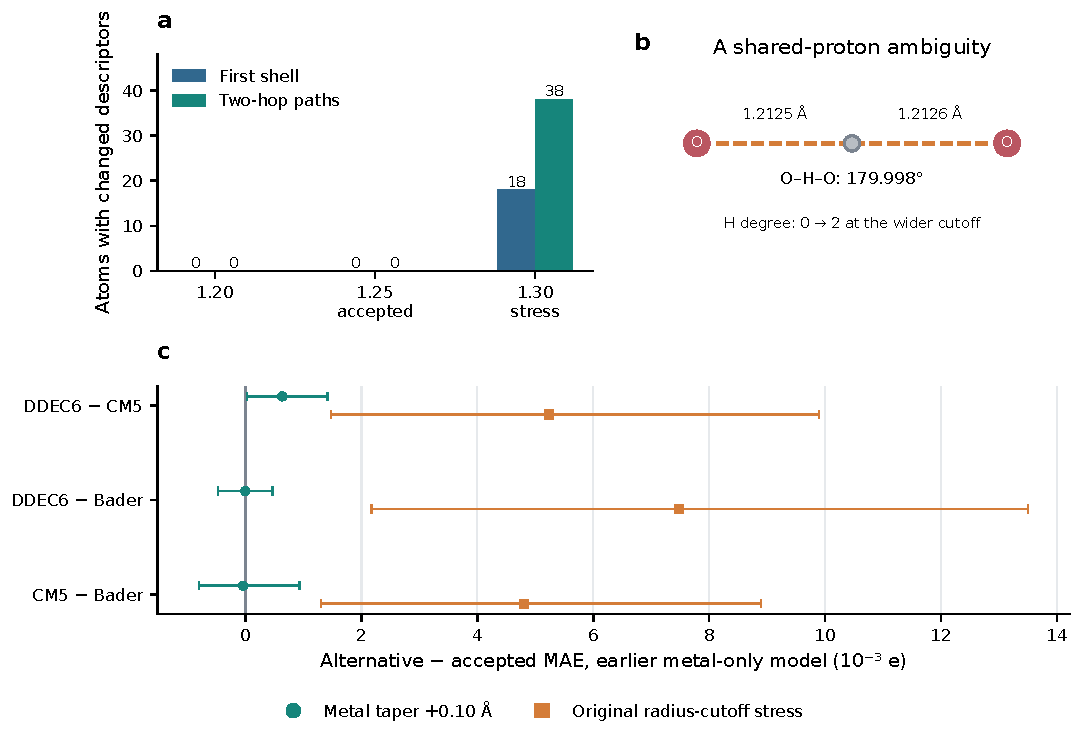
\includegraphics[width=\textwidth]{figures/Figure_05_connectivity_limits.pdf}
\caption{\textbf{Connectivity stability and ambiguity are distinct.} (a) Atoms with changed first-shell or two-hop features under nonmetal cutoff scales 1.20 and 1.30 relative to 1.25, on 96 structures containing 16,165 atoms; metal-involving edges are fixed. (b) One recorded near-midpoint O--H--O geometry, reconstructed from its saved distances and angle. Dashed contacts are added by the wider stress cutoff; the drawing is a local geometry illustration, not a bond-truth assignment. Six H sites exhibit this ambiguity. (c) Earlier fixed metal-only two-hop model sensitivity to a shifted metal distance taper and to the original radius-cutoff stress graph, using 508 metal atoms on the 96-structure subset. Error bars are the saved pointwise 95\% structure-bootstrap intervals. Panel (c) is explicitly an earlier model diagnostic and must not be read as a refit or sensitivity test of the final charge-conditioned models.}
\label{fig:graph}
\end{figure}

\FloatBarrier
\subsection{Interpretation and limits}
The combined evidence supports a chemical organization of charge-definition disagreement within the tested cohort. It does not identify a preferred universal charge scale. Absolute departures quantify the failure of an empirical mapping, while within-environment residual spread describes heterogeneity around that mapping. Neither quantity has been calibrated against a physical charge error or a downstream experimental observable. Likewise, related-record blocking and graph perturbation constrain particular explanations of the result without establishing broad chemical-family transfer or universal bonding correctness.

The atlas can guide inspection of a charge mapping by identifying environments with a directional offset, elevated absolute departure, or heterogeneous residuals. It supplies paired support and ambiguity coverage for that inspection. The carbon examples demonstrate a chemical organization of the differences, but attachment labels alone do not isolate polarization, resonance, or another electronic mechanism. Likewise, the metal failure identifies a limit of the present population and representation without showing that metal chemistry is absent. Connecting any atlas pattern to adsorption performance or another observable requires a separate application-specific test.
